\subsubsection{28.01.2016}
\textit{\textbf{Time frame:}} 17:00-22:00 

It was started the development of the protection of the servos' wires on the bucket from grasping the elements of construction while shifting.

It was also created a protection from the engagement of the cable with the axis at the mechanism for shifting the bucket.

\begin{figure}[H]
	\begin{minipage}[h]{0.47\linewidth}
		\center{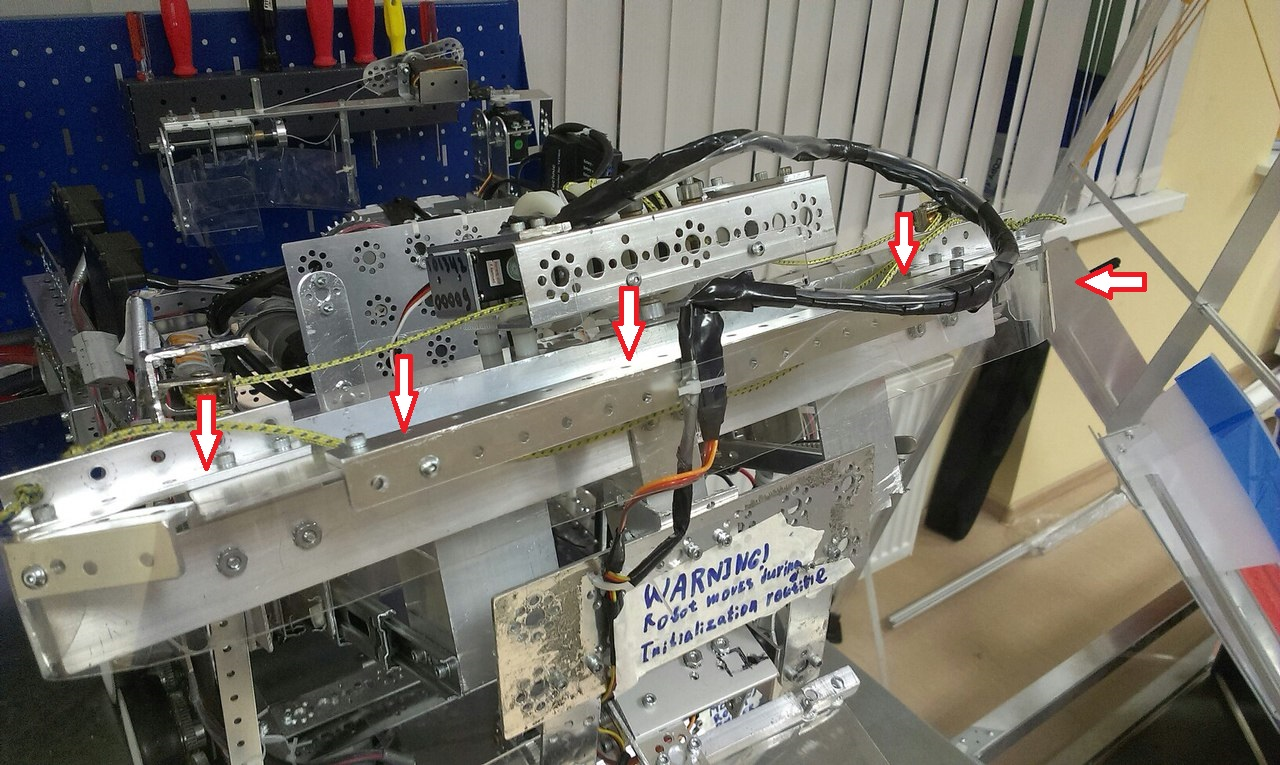
\includegraphics[scale=0.2]{3Engineering/5Team_meetings/days_of_meetings/2016.01.28/images/01}}
		\caption{Protection for wire}
	\end{minipage}
	\hfill
	\begin{minipage}[h]{0.47\linewidth}
		\center{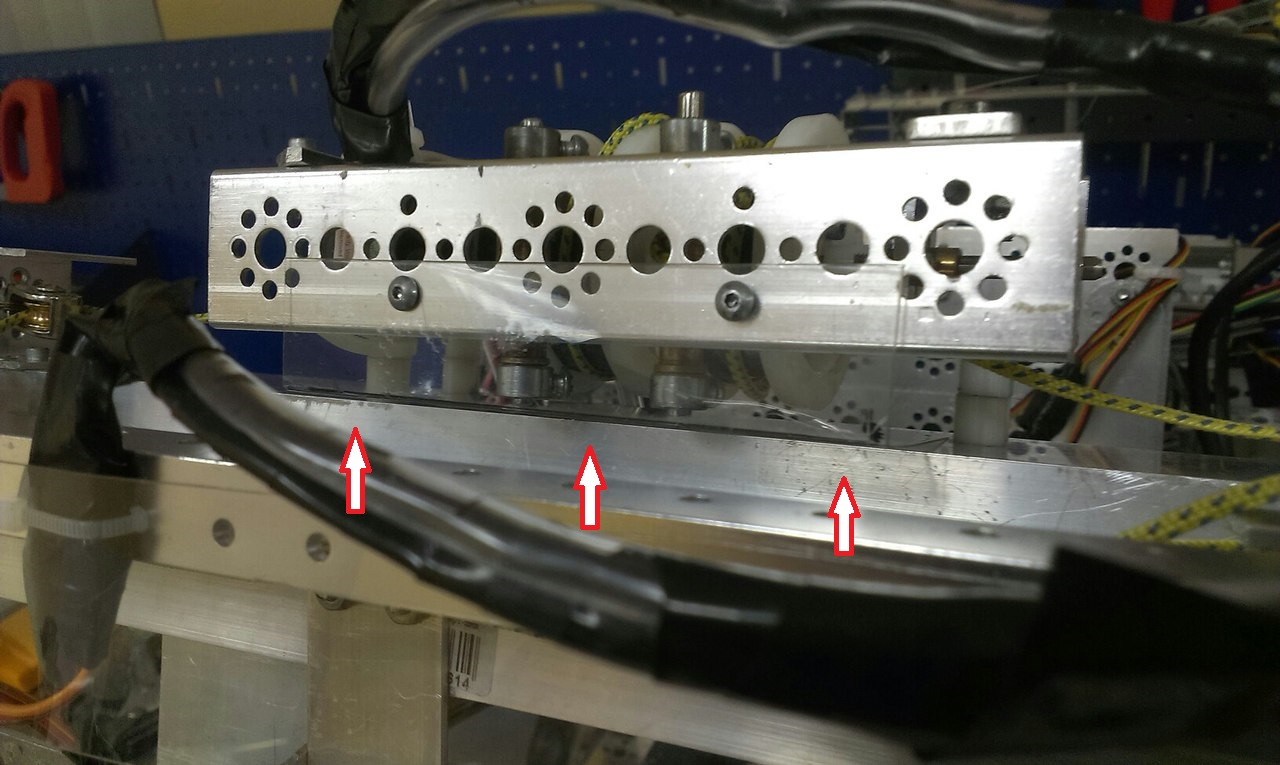
\includegraphics[scale=0.2]{3Engineering/5Team_meetings/days_of_meetings/2016.01.28/images/02}}
		\caption{Protection for cables}
	\end{minipage}
\end{figure}

The mount of the second block on the elevator was strethened.

%\begin{figure}[H]
%	\begin{minipage}[h]{1\linewidth}
%		\center{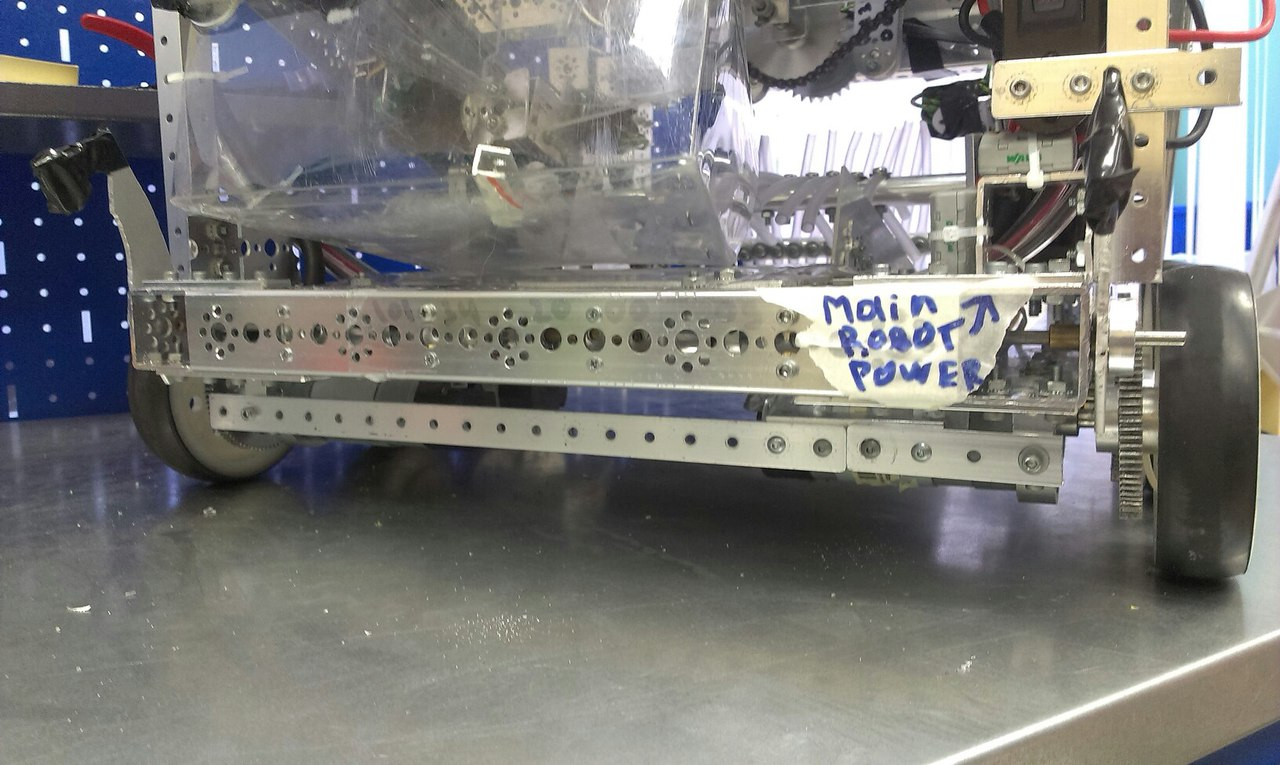
\includegraphics[scale=0.2]{3Engineering/5Team_meetings/days_of_meetings/2016.01.28/images/03}}
%		\caption{The mount of the block}
%	\end{minipage}
%\end{figure}

It was started the creating of the borders at the sides of a gripper, that will prevent debris from getting into the areas beyond these borders. There were taken all the needed measurements. After that, a part of these borders was cut out from PET.